\section{Implementierung}


\subsection{Probleme} \label{Probleme}

\begin{enumerate}
    \item Taxi\\
    Für das Taxiproblem wurde ein fünf mal fünf großen Feld implementiert, der Agent (Taxifahrer) hat dabei die Möglichkeit, sich in alle vier Himmelsrichtungen zu bewegen. Die Aufgabe besteht darin, den Passagier, welcher sich in einer zufälligen Ecke des Feldes befindet, abzuholen und ihn dann zu seinem gewünschten Ziel zu bringen. Das gewünschte Ziel des Passagiers ist immer einer der verbleibenden Ecken des Spielfeldes. Um diese Aufgabe noch etwas zu erschweren, wurden zusätzlich noch Wände in das Feld mit integriert. Diese befinden sich immer an den gleichen Positionen und verhindern Bewegungen in bestimmte Richtungen.

    Für das Bewältigen dieser Aufgabe kann der Agent zu jedem Zeitpunkt zwischen sechs Actions entscheiden; Bewegung in jeweils einer der vier Himmelsrichtungen, aufnehmen des Passagiers und das Absetzen des Passagiers. Natürlich sind nicht alle Actions zu jedem Zeitpunkt sinnvoll. 

    Der Zustand des Feldes kann durch 500 diskrete States beschrieben werden. Diese Anzahl ergibt sich aus der Multiplikation der 25 möglichen Position des Taxis, der fünf möglichen Positionen des Passagiers (beinhaltet den Fall, dass sich der Passagier im Taxi befindet), mit den vier möglichen Zielorten.

    Da das Abliefern des Passagiers an dem richtigen Strandort das Ziel der Aufgabe ist, bekommt der Agent dafür auch die höchste Belohnung. Damit die Erfüllung der Aufgabe so effizient wie möglich durchgeführt wird, bekommt der Agent für jede Action, die er durchführt und die nicht zu einer Belohnung führt, eine kleine Strafe. Zuletzt wird der Agent stark bestraft, wenn er den Passagier an dem falschen Ort absetzt oder versucht, einen Passagier an einer falschen Position aufzunehmen.
    \begin{figure}
        \centering
        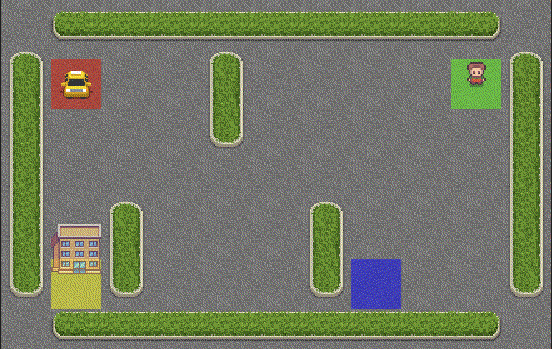
\includegraphics[scale=0.7]{taxi}
        \caption{Taxi Environment}
        \label{fig:taxi_env}
    \end{figure}
    
    
    \item Cliff\\
    Wie für das Taxiproblem wurde auch für das Cliff Walking Problem ein Feld implementiert, dieses Mal allerdings in der Größe von vier mal zwölf. Die Aufgabe des Agenten besteht darin, von einer Seite des Feldes zur anderen zu gelangen, ohne dabei in die auf dem Feld befindliche Kippe zu fallen. Als Klippe wurden alle Felder definiert, welche sich auf dem direkten Weg zwischen Agent und Ziel befinden. Der Agent hat somit die Aufgabe, um diese Klippe herum zu navigieren und so das Ziel zu erreichen. Um die Herangehensweise der verschiedenen Algorithmen besser vergleichen zu können, befinden sich bei diesem Experiment alle Objekte (Agent, Klippen, Zielpunkt) zu Beginn jeder Episode an derselben Position.

    Damit sich der Agent auf dem Feld bewegen kann, stehen ihm vier verschiedene Actions zur Verfügung, welche den Agent jeweils um ein Feld in einer der Himmelsrichtungen verschiebt.

    Um den Zustand des Environments zu beschreiben, ist die aktuelle Position des Agent ausreichend. Insgesamt gibt es 48 (4 × 12) verschiedene Positionen auf dem Feld. Da das Betreten des als Kippe definierten Bereiches jedoch zum Ende der Episode führt, sind diese Positionen kein gültiger State. Gleiches gilt auch für die Zielposition. Bei zehn Klippen und einem Ziel ergeben sich so 37 States.

    Neben des Erreichen des Ziels ist es besonders wichtig, dass der Agent nicht in die Klippe fällt, daher ist dies mit einer hohen Bestrafung für den Agent versehen. Zudem soll das Ziel so schnell wie möglich erreicht werden, daher ist, wie auch bei Taxi Problem, jede Action mit einer kleinen Strafe belegt. Eine explizite Belohnung des Agent ist für diesen Anwendungsfall nicht nötig, da das Ziel zur Beendung der Episode führt und das beste Ergebnis somit das ist, welches zur geringsten Bestrafung führt.

    \begin{figure}
        \centering
        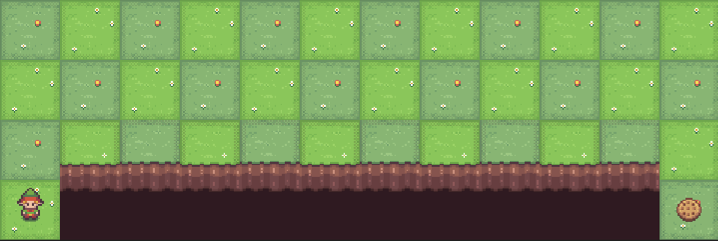
\includegraphics[scale=0.7]{cliff}
        \caption{Cliff Environment}
        \label{fig:cliff_env}
    \end{figure}
    
    \item Frozen Lake\\
    Auch das Frozen Lake Problem ist auf einem Gitternetz aus Feldern implementiert. Einige Felder sind Eisplatten, die der Agent sicher betreten kann, während andere Felder Löcher darstellen, in die der Agent fallen kann und damit das Spiel verliert. Das Ziel des Agenten besteht darin, sicher zum Ziel zu gelangen, welches sich auf der anderen Seite des Sees (Gitternetz) befindet. Die besondere Herausforderung bei diesem Problem sind die Eisplatten, bewegt sich der Agent auf einer dieser Platten in eine bestimmte Richtung besteht eine Change, dass der ausrutscht und sich in eine andere Richtung bewegt.

    Wie auch beim Cliff Problem kann der Agent nur durch Bewegung mit dem Environment interagieren und hat somit vier Actions zur Verfügung.

    Eine weitere Herausforderung besteht darin, dass die Positionen der Löcher nicht fest sind, sondern bei Beginn jeder Episode zufällig festgelegt werden. Dies muss beim Abbilden des Zustandes des Environments als States berücksichtigt werden. Ein vier mal vier großes Environment mit drei Löchern hat somit 4368 mögliche States. Dies setzt sich zusammen aus den 12 möglichen Positionen des Agenten (16 Felder minus die Löcher und des Ziels) multipliziert mit den 364 möglichen Kombinationen, die 3 Löcher auf 14 freie Flächen zu verteilen.

    Die Struktur des Rewards ist für dieses Problem recht simpel, der Agent wird belohnt, wenn er das Ziel erreicht und bestraft, wenn er in ein Loch fällt.
    
    \begin{figure}
        \centering
        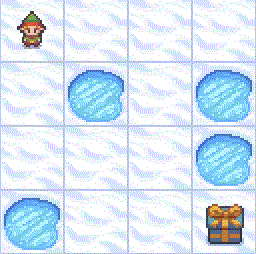
\includegraphics[scale=0.7]{frozen_lake}
        \caption{Frozen Lake Environment}
        \label{fig:frozen_env}
    \end{figure}


\end{enumerate}

\subsection{Optimierung der Hyperparameter}
Die Theoretischen Grundlage der Hyperparameter wurde bereits in \ref*{Def_Hyperparameter} \nameref{Def_Hyperparameter} erläutert, um konkreten Werte für die im Rahmen dieser Arbeit untersuchten Problem zu finden, wurden einige Versuche durchgeführt. 
Als Ausgangslage wurde die in \nameref{tab:hyperBasic} dargestellten Werte angenommen. Im Folgenden werden diese initialen Werte anhand von Experimenten für die verschiedenen Algorithmen und Probleme optimiert.

\begin{table}[h]
    \caption{Hyperparameter Ausgangslage}
    \label{tab:hyperBasic}
    \centering
    \rowcolors{2}{white}{lightgray} 
    \begin{tabular}{>{\itshape}0l0l}\hline % used >{\itshape} in order to be able to remove the repeated occurences of \textit in the first column, used l type columns instead of c columns for a cleaner look, added small vertical space above and below the rows with the help of the cellspace package, removed all vertical lines
    \textup{Paramater}          & Wert\\\hline
    num\_episodes               & 1000\\
    max\_steps\_per\_episode    & 1000\\
    learning\_rate              & 0.1\\
    discount\_rate              & 0.99\\
    exploration\_rate           & 1\\
    max\_exploration\_rate      & 1\\
    min\_exploration\_rate      & 0.01\\
    exploration\_decay\_rate    & 0.005\\\hline
    \end{tabular}
\end{table}

\begin{itemize}
    \item Anzahl an Episoden\\
    Als optimale Anzahl an Episoden wird der Punkt gewählt, ab wann sich der Agent nicht mehr verbessert, so wird ein unnötig langes Training vermieden. 
    Dieser Punkt lässt sich sehr gut in einer grafischen Darstellung der erreichten Belohnung des Agenten im Vergleich zu den während des Trainings durchlaufenen Episoden ablesen. 
    Die Rohdaten aus dem Training sind aufgrund der Exploration sehr verrauscht, und der eigentliche Trainingsfortschritt ist nur schwer zu erkennen.
    Um die Grafik lesbarer zu machen wurde ein gleitender Durchschnitt auf die Daten angewandt, der Effekt dieser Operation wurde in der Abbildung \nameref{fig:NumOfEpisods_Taxi} veranschaulicht.

    \begin{figure}[H]
        \centering
        \begin{subfigure}{.5\textwidth}
          \centering
          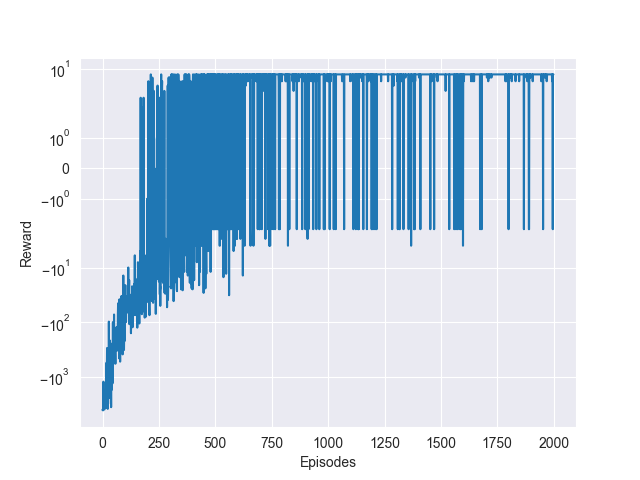
\includegraphics[width=1\linewidth]{Hyper_Data_Raw}
          \caption{Rohdaten}
          \label{fig:NumOfEpisods_Raw}
        \end{subfigure}%
        \begin{subfigure}{.5\textwidth}
          \centering
          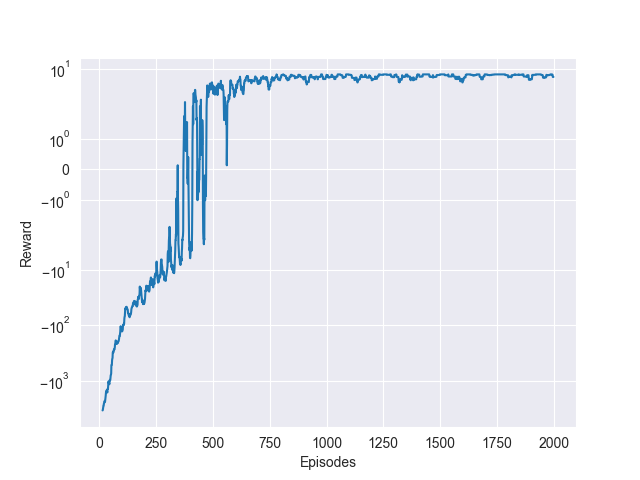
\includegraphics[width=1\linewidth]{Hyper_Data_Clean}
          \caption{Gleitender Durchschnitt}
          \label{fig:NumOfEpisods_clean}
        \end{subfigure}
        \caption{Anwendung gleitender Durchschnitt}
        \label{fig:NumOfEpisods_MovingAVG}
    \end{figure}

    \item Maximale Anzahl an Steps pro Episode\\
    Für die Festlegung dieses Hyperparameters wurde zunächst der Trainingsverlauf der Basiswerte mit dem Trainingsverlauf von deutlich erhöhten und reduzierten Werten verglichen.
    So konnte der Einfluss des Parameters analysiert werden und eine erste Tendenz wurde festgestellt.
    Darauf folgenden weitere Vergleiche, um den optimalen Wert zu bestimmen.

    \item Learning Rate\\
    Wie auch bei der Festlegung der maximalen Anzahl an Steps pro Episode wurde auch für die Learning Rate der initiale Wert verändert und die Auswirkungen anhand von Grafen analysiert.

    \item Discount Rate\\
    Die Discount Rate wurde ebenfalls ermittelt, indem die Auswirkungen einer Veränderung des Hyperparameters untersucht wurden. 
    Der initial gewählte Wert für die Discount Rate ist sehr nah am Maximum des möglichen Wertebereichs. 
    Das Erhöhen dieses Hyperparameter führte daher in keinem Versuch zu einer Veränderung der Ergebnisse. 
    Die Reduzierung des Parameters wirkte sich jedoch auf das Training des Agenten aus.

    \item Exploration Rate\\
    Damit sich der Wert der Exploration Rate über den Verlauf des Trainings verändert, sind insgesamt vier Parameter implementiert. 
    Die Obergrenze für den Wert, sowie der Startwert, sind initial auf Eins festgelegt. 
    Zu Beginn hat der Agent noch kein Wissen über das Environment, eine Exploitation ist somit nicht sinnvoll. 
    Eine Reduzierung des Wertes führt somit nur zu einem langsamen Trainingsverlauf. 
    Die Obergrenze soll den höchsten erreichbaren Wert beschreiben, da die Exploration Rate während des Trainings ausschließlich reduziert wird, muss dieser Wert mit dem Startwert identisch sein.
    Die Abnahmerate und der minimale Wert sind durch Experimente werten, wie die vorherigen drei Hyperparameter durch Versuche ermittelt.
\end{itemize}


\subsection{Vergleichen von Algorithmen}

Nach dem im vorangegangen Kapitel die Implementation des Vergleichens der Hyperparameter beschrieben wurde, befasst sich dieser Abschnitt mit dem Verlgeichen der beiden Algorithmen Q-Learning und SARSA. 
Um den bestmöglichen Vergleich zu gewährleisten wurden geeignete Parameter für beide Algorithmen und die jeweiligen Probleme gewählt. Bei der Analyse wurden alle drei Probleme, welche in \ref{Probleme} bereits erläutert wurden, angewendet.


\begin{itemize}
    \item Bei dem Taxiproblem wurden die in Tabelle \ref{tab:Taxi} dargestellten Paramater für einen sinnvollen Vergleich der beiden Algorithmen gewählt. Das Taxi-Problem hat im Vergleich zu den anderen Algorithmen viele unterschiedliche States, daher brauche es eine hohe Anzahl an Episoden um diese zu lernen bzw. zu optimieren.
    
    \item Bei dem Cliffproblem handelt es sich um ein einfacheres Problem, daher wurden die Anzahl der Episoden etwas zurückgesetzt. Die für dieses Problem genutzten Parameter sind in Tabelle \ref{tab:Cliff} beschrieben.
    
    Die Besonderheit bei dem Cliffproblem ist, dass es lediglich negative Belohnungen gibt und die Klippe eine vielfach höhere Bestrafung hat, als ein normaler Schritt, welcher nicht die Klippe hinunter führt. 

    \item Bei dem Frozen Lake Problem handelt es sich widerum um ein komplexeres Problem, welches mehr Episoden als das Cliffproblem benötigt, um zu einem Optimum zu konvergieren. Wichtig bei diesem Problem ist ebenfalls eine höhere Anzahl an maximalen Steps, bevor der Algorithmus in die nächste Episode geht. 
    Der Grund dafür ist, dass es lediglich für das Zielfeld als Belohnung +1 gibt, während alle anderen Aktionen im Spiel mit dem Reward 0 belegt sind. Somit muss der Agent es über die Exploration erstmal schaffen das Zielffeld zu entdecken, um sich dann im nachhinein dafür zu optimieren. 
    Erschwert wird das ganze zusätzlich durch die Tatsache, dass neben der Exploration Rate (epsilon) auch das Environment für zufällige Bewegungen sorgt. So ist die Wahrscheinlichkeit, wenn der Agent nach links gehen möchte lediglich P(links) = 1/3 und die Chancen für die Richtungen oben und unten auch jeweils P(oben) = 1/3 und P(unten) = 1/3. 
    Die Tabelle \ref{tab:FrozenLake} führt die genutzten Parameter für den Vergleich von Q-Learning und SARSA dieses Problems auf.
   
    \begin{table}[!htb]
        % \caption{Global caption}
        \begin{minipage}{.5\linewidth}
            \caption{Taxi Paramater}
            \label{tab:Taxi}
            \centering
            \rowcolors{2}{white}{lightgray} 
            \begin{tabular}{>{\itshape}0l0l}\hline % used >{\itshape} in order to be able to remove the repeated occurences of \textit in the first column, used l type columns instead of c columns for a cleaner look, added small vertical space above and below the rows with the help of the cellspace package, removed all vertical lines
            \textup{Paramater}          & Wert\\\hline
            num\_episodes               & 3000\\
            max\_steps\_per\_episode    & 1000\\
            learning\_rate              & 0.1\\
            discount\_rate              & 0.99\\
            exploration\_rate           & 1\\
            max\_exploration\_rate      & 1\\
            min\_exploration\_rate      & 0.05\\
            exploration\_decay\_rate    & 0.005\\\hline
            \end{tabular}
        \end{minipage}%
        \begin{minipage}{.5\linewidth}
            \caption{Cliff Paramater}
            \label{tab:Cliff}
            \centering
            \rowcolors{2}{white}{lightgray} 
            \begin{tabular}{>{\itshape}0l0l}\hline % used >{\itshape} in order to be able to remove the repeated occurences of \textit in the first column, used l type columns instead of c columns for a cleaner look, added small vertical space above and below the rows with the help of the cellspace package, removed all vertical lines
            \textup{Paramater}          & Wert\\\hline
            num\_episodes               & 1500\\
            max\_steps\_per\_episode    & 1000\\
            learning\_rate              & 0.1\\
            discount\_rate              & 0.99\\
            exploration\_rate           & 1\\
            max\_exploration\_rate      & 1\\
            min\_exploration\_rate      & 0.05\\
            exploration\_decay\_rate    & 0.005\\\hline
            \end{tabular}
        \end{minipage} 
    \end{table}

    \begin{table}[h]
        \caption{Frozen Lake Paramater}
        \label{tab:FrozenLake}
        \centering
        \rowcolors{2}{white}{lightgray} 
        \begin{tabular}{>{\itshape}0l0l}\hline % used >{\itshape} in order to be able to remove the repeated occurences of \textit in the first column, used l type columns instead of c columns for a cleaner look, added small vertical space above and below the rows with the help of the cellspace package, removed all vertical lines
        \textup{Paramater}          & Wert\\\hline
        num\_episodes               & 2000\\
        max\_steps\_per\_episode    & 10000\\
        learning\_rate              & 0.1\\
        discount\_rate              & 0.99\\
        exploration\_rate           & 1\\
        max\_exploration\_rate      & 1\\
        min\_exploration\_rate      & 0.05\\
        exploration\_decay\_rate    & 0.005\\\hline
        \end{tabular}
    \end{table}
\end{itemize}

Zum Vergleich der Algorithmen wurden die Belohnungen und Steps während des Trainings aufgenommen und anschließend in Plots anschaulich dargestellt. 
Dabei wurde je nach Problem eine logarithmische Skalar auf der y-Achse genutzt, um die Daten anschaulicher zu machen. Zusätzlich wird ein Rolling Window Ansatz gewählt, sodass immer 15 Werte zusammengefasst werden. Dies sorgt dafür das einzelne Peaks zwar weniger auffallen, dafür der Gesamttrend im Verlauf der Trainingsepisoden aber besser zu erkennen ist.


    
